In der Abbildung \ref{fig:dateflowVScodedep} ist ein Beispiel von einer Anwendung zu sehen, die die von der Konsole ankommenden Zahlen quadriert und das Ergebnis zurückgibt.
                
\begin{figure}[H]
    \centering
    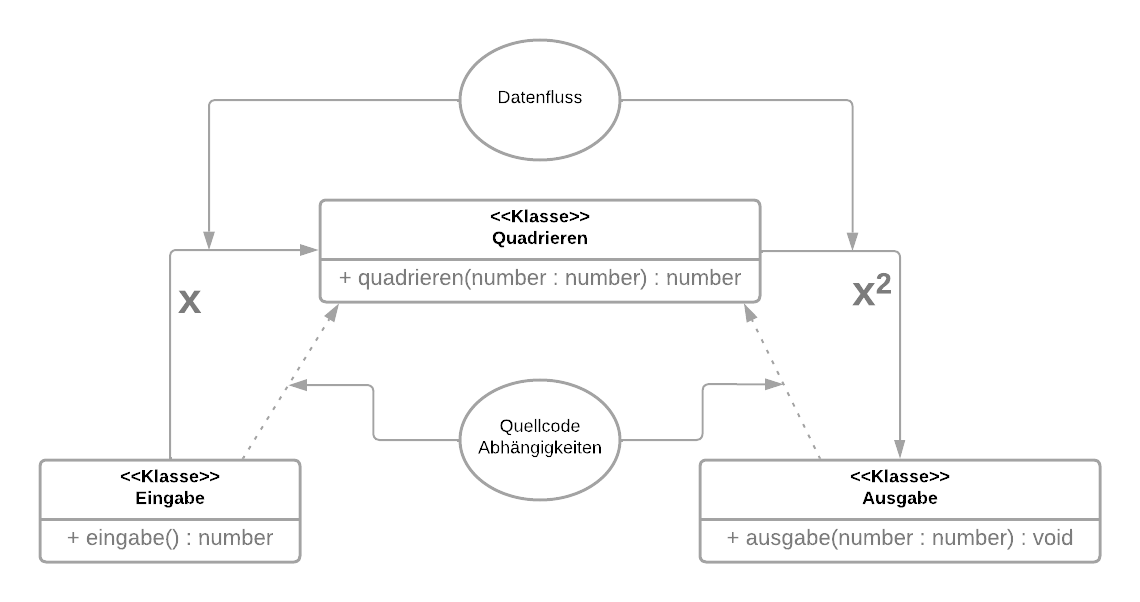
\includegraphics[width=1\textwidth]{./images/DepInj_1.png}
    \caption{Datenfluss und Quellcode Abhängigkeiten}
    \label{fig:dateflowVScodedep}
\end{figure}

Die Funktion \textbf{Quadrieren} befindet sich in dem Fall auf einem höheren Niveau als Eingabe und Ausgabe, 
da das Quadrieren einer Zahl unabhängig von der Eingabe und Ausgabe sein soll.

Wenn die Eingabeparameter bei der Ausgabe von \textbf{number} auf \textbf{string} geändert wird, 
muss die Ausgabe von Quadrieren von \textbf{number} auf \textbf{string} geändert werden.
Dadurch kann auch eine weitere Kette an Anderungen im Programm ausgelöst werden. 
Zum Beispiel müssen auch die Unittests von \textbf{Quadrieren} geändert werden.
Somit ist \textbf{Quadrieren} abhängig von der \textbf{Ausgabe}

Das Problem lässt sich mittels Dependency Injection lösen.
In OOP Sprachen lässt sich dafür ``Interface'' benutzen.

Die Lösung sieht so aus: 
\begin{figure}[H]
    \centering
    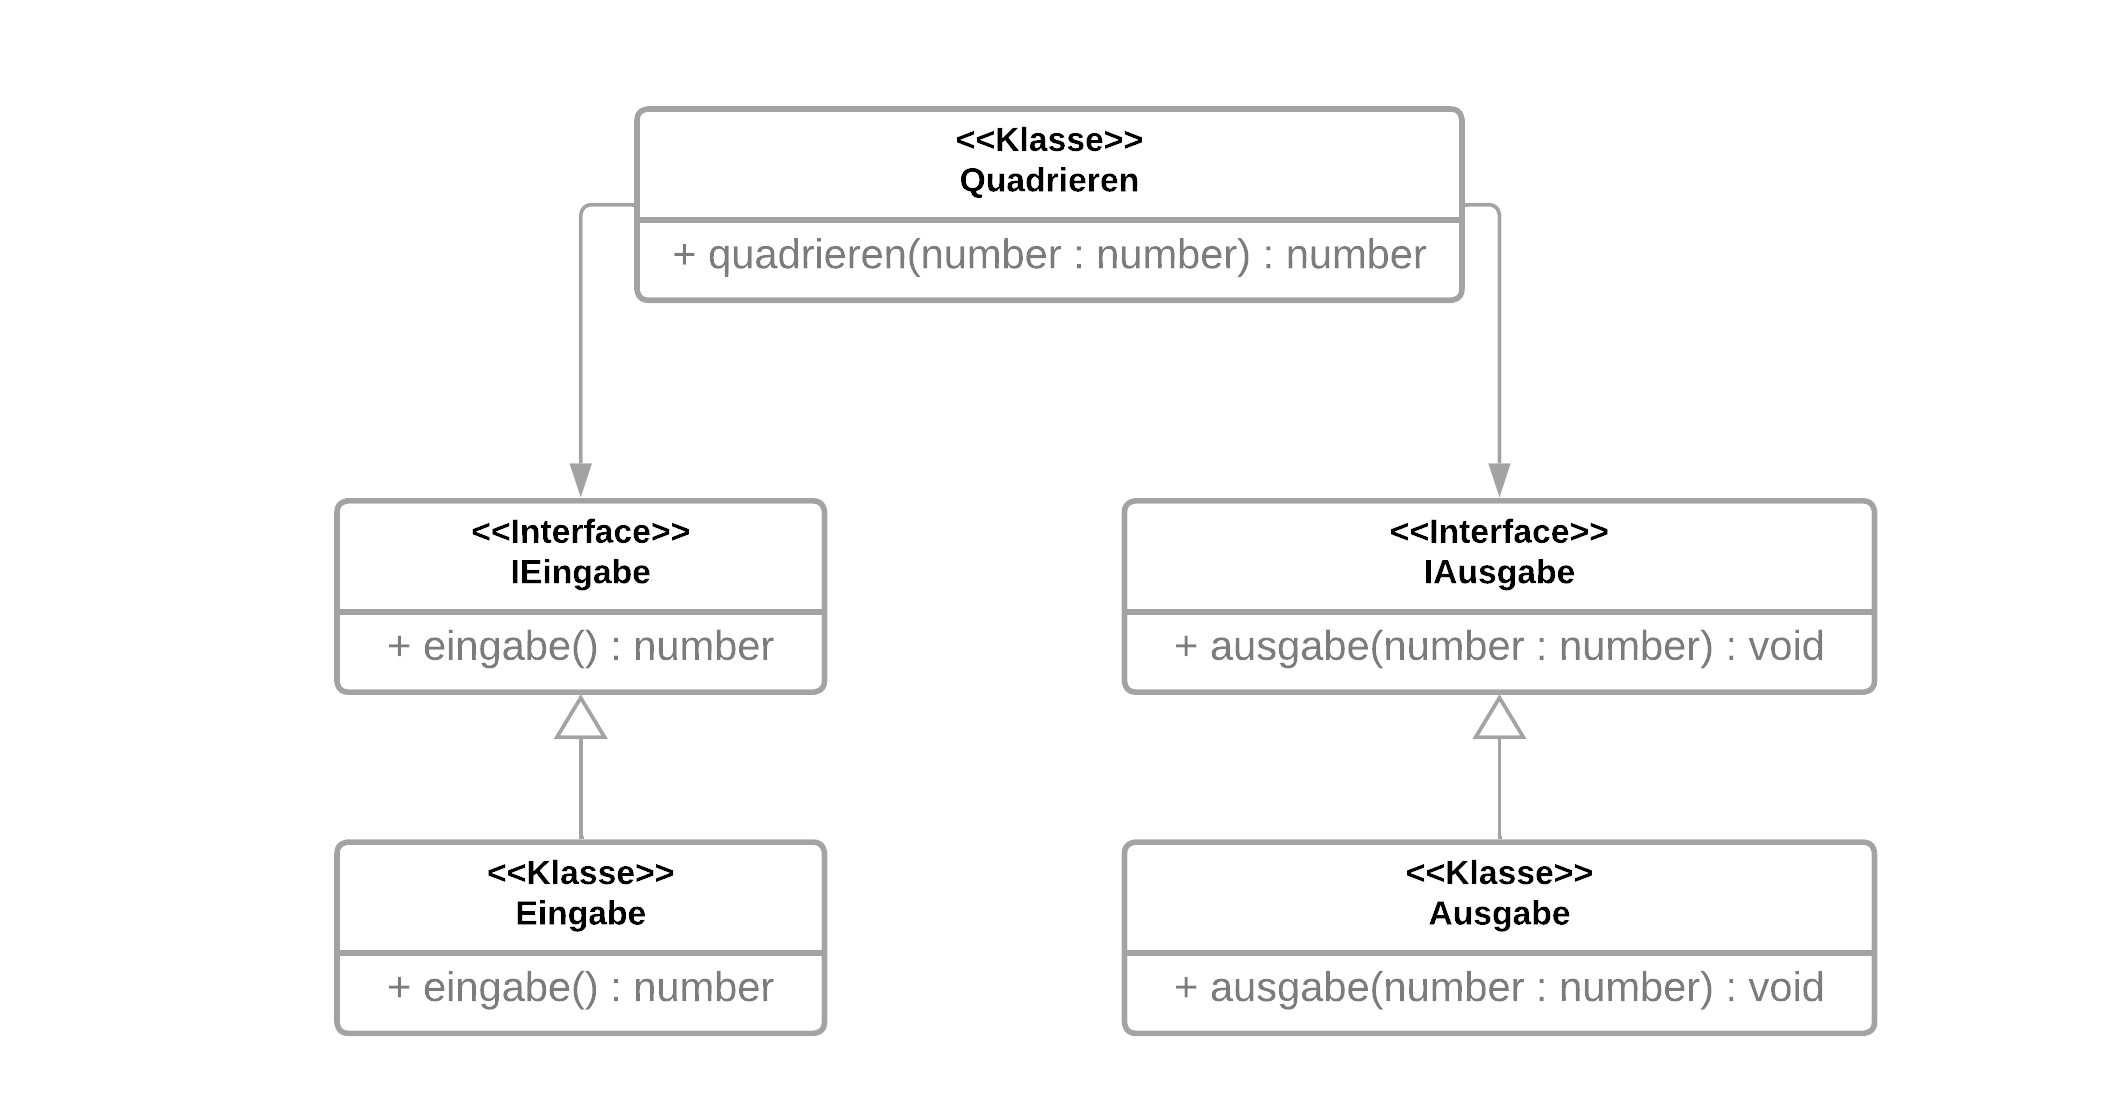
\includegraphics[width=1\textwidth]{./images/DepInj_2.png}
    \caption{Entkopplung der Abhängigkeiten}
    \label{fig:flow around cylinder}
\end{figure}

Dies lässt sich mit \textbf{Interface} (für OOP Sprachen) umsetzen, 
in dem es frühestens bei der Initialisiereung der \textbf{Quadrieren} 
Klasse das jeweilige Eingabe und Ausgabe Objekt übergeben wird.

Somit lässt sich die Funktion \textbf{Quadrieren} mit gefälschten Eingabe- und Ausgabeklasse mit Unit tests getestet werden.

Wenn alle Klassen über Interface miteinander verbunden sind, 
ist es möglich, dass die Umgebung von jeder einzelnen Klasse bei den Unittests gefälscht
wird und somit das Schreiben von Unittests sehr einfach wird. 

Interfaces können sich auch ändern und dann müssen alle davon betroffenen Objekte entsprechend geändert werden, 
jedoch passiert das deutlich seltener als Änderung einer Klasse.

Auch mit Dependency Injection lassen sich externe Schnittstellen wie Datenbank oder Netzwerkschnittstellen schnell austauschen, 
denn es ist nur eine Klasse zu schreiben, die das Interface implementiert.